\chapter{Basic Concepts \& System Structure}
\label{ch:struct}
In order to warrant the sizeable effort designing and constructing an entire OS from scratch,
basic concepts need be novel. The principal concepts underlying Oberon and the dominant
design decisions are 1st discussed. Upon this, the system structure was then presented,
restricted to the coarsest, the composition and interdependence of the largest building
blocks, \emph{modules}. Finally, an overview, helps understanding the place, role, and
significance of each part (chapter).

The fundamental OS objective is to present the computer at a certain abstraction level
to the user and programmer. For example,
\begin{description}
  \item[~~~~~~store] requestable \emph{variables} of a specified data type,
  \item[~~~~~~~~disk] sequences of characters or bytes called \emph{files},
  \item[~~~display] rectangular areas called \emph{viewers},
  \item[keyboard] an \emph{input stream} of characters, and
  \item[~~~~~mouse] a pair of \emph{coordinates} and a set of \emph{key states}.
\end{description}
Every abstraction is characterized by certain \emph{properties} and governed by a set of
\emph{operations}. It is the \emph{task} of OS to implement these operations and to manage
them, constrained by the available resources of the underlying computer. This is commonly
called \emph{resource management} (RM).

Every abstraction inherently hides details, from which it abstracts. Hiding occurs
at different levels. For example, the
\begin{itemize}
  \item computer may make certain store parts or devices inaccessible
    according to operation modes (user/supervisor);
  \item programming language may make certain parts inaccessible through a facility
    inherent in visibility rules.
\end{itemize}
The latter is of course much more flexible and powerful, while the former indeed plays an
almost negligible role in our system. Hiding is important because it allows maintenance
of certain properties (called \emph{invariants}) of an abstraction to be guaranteed.
Abstraction is indeed the key of any modularization, and without it every hope of being
able to guarantee reliability and correctness vanishes. Clearly, Oberon was designed with
the goal of establishing a modular structure on the basis of purpose-oriented abstractions.
The availability of an appropriate programming language is an indispensable prerequisite,
and the importance of prudent choice cannot be over-emphasized.

\section{Concepts}
\subsection{Viewers}
Whereas the abstractions of individual variables representing parts of the primary store,
and of files representing parts of the disk store are well established notions and have
significance in every computer system, abstractions regarding input and output devices
became important with the advent of high interactivity between user and computer. High
interactivity requires high bandwidth, and the only channel of human users with high
bandwidth is the eye. Consequently, the computer's visual output unit must be properly
matched with human eyes. This occurred with the advent of the \emph{high-resolution
display} (HRD) in the mid 1970s, which in turn had become feasible due to faster and
cheaper electronic memory components. The HRD marked one of the few very significant
break-throughs in the history of computer development. The typical bandwidth of a modern
display is in the order of 100 MHz. Primarily the HRD made visual output a subject of
abstraction and RM. In Oberon, the display is partitioned into \emph{viewers}, also called
windows, or more precisely, \emph{frames}, rectangular areas of the screen(s). A viewer
typically consists of:
\begin{description}
  \item[title bar] contains a subject name and commands menu,
  \item[main frame] some text, graphic, video, or other object.
\end{description}
Viewers (frames) can be nested, in principle to any depth.

\verb|System| provides routines for generating, moving, and closing a viewer. It allocates
a new one at a specified place, and upon request delivers hints as to where it might best
be placed. It keeps track of their opened set. These are called \emph{viewer management},
in contrast to contents handling.

High interactivity requires not only high visual output bandwidth but also input flexibility.
Surely, there is no need for an equally high bandwidth, but a \textbf{keyboard} limited by
the speed of typing to about 100 Hz is not good enough. The break-through on this front was
achieved by a pointing device, \textbf{mouse}, appeared roughly the same time as HRD.

This was by no means just a lucky coincidence. The mouse comes to fruition only through
HRD and appropriate software. It is itself a conceptually very simple device delivering
signals when moved on the table. These signals allow the computer to update the position of
a mark - the cursor - on the display. Since feedback occurs through human eyes, no great
precision is required. For example, when the user wishes to identify a certain object, e.g.
a letter on the screen, one moves the mouse as far as required until the mapped cursor
reaches the object. This stands in marked contrast to a digitizer which is supposed to
deliver exact coordinates. Oberon relies highly on it.

Perhaps the cleverest idea was to equip mice with buttons. By being able to signal a request
with the same hand that determines the cursor position, the user obtains the direct impression
of issuing position-dependent requests. Position-dependence is realized in software by
delegating interpretation of the signal to a procedure - a so-called handler or interpreter
- which is local to the viewer in whose area the cursor momentarily appears. A surprising
flexibility of command activation can be achieved in this manner by appropriate software.
Various techniques have emerged in this connection, e.g. pop-up menus, pull-down-menus, etc.
which are powerful even under the presence of a single button only. For many applications,
a mouse with several keys is far superior, and Oberon basically assumes 3 buttons to be
available. The assignment of different functions to the keys may of course easily lead to
confusion when every application prescribes different key assignment. This is, however,
easily avoided by the adherence to certain "global" conventions. In Oberon, button of the:
\begin{description}
  \item[left] primarily used for marking a position (setting a caret),
  \item[middle] for issuing general commands (see below), and
  \item[right] for selecting displayed objects.
\end{description}

Recently, it has become fashionable to use overlapping windows mirroring documents being
piled up on the desktop. We have found this metaphor not entirely convincing. Partially
hidden windows are typically brought to the top and made fully visible before any operation
is applied to their contents. In contrast to the insignificant advantage stands the
substantial effort necessary to implement this scheme. It is a good example of a case
where the benefit of a complication is incommensurate with its cost. Therefore, we have
chosen a solution that is much simpler to realize yet has no genuine disadvantages:
\emph{tiled viewers} as shown in Fig \ref{fig:viewers}:
\begin{figure}[h!]
  \centering
  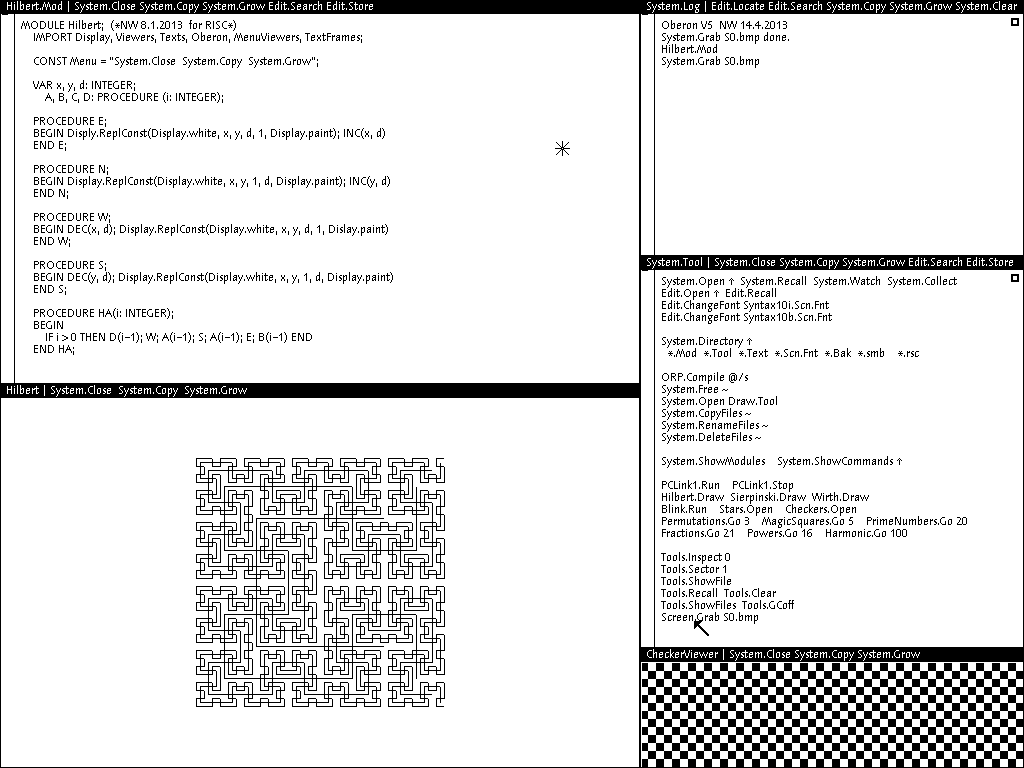
\includegraphics[width=.75\textwidth]{i/1.png}
  \caption{Oberon display with tiled viewers}
  \label{fig:viewers}
\end{figure}

\subsection{Commands}
Position-dependent commands with meaning fixed for each type of viewer must be supplemented
by general commands. Conventionally, such commands are issued through the keyboard by
typing the program's name that is to be executed into a special command text. In this
respect, Oberon offers a novel and much more flexible solution:
\begin{itemize}
  \item[$1^{st}$] of all we remark that a program in the common sense of a text compiled
as a unit is mostly a far too large action unit to serve as a command. Compare it with,
for example, the insertion of a piece of text through a mouse command. In Oberon, the
notion of a action unit is separated from the notion of compilation unit. The former is a
command represented by a (exported) procedure, the latter a module. Hence, a module may,
and typically does, define several, even many commands. Such a (general) command may be
invoked at any time by pointing at its name in any text visible in any viewer on the display,
and by clicking the middle mouse button. The command name has the form \verb|M.P|, where
\verb|P| is the procedure's identifier and \verb|M| the module in which \verb|P| is declared.
As a consequence, any command click may cause the loading of one or several modules, if
\verb|M| is not already present in main store. The next invocation of \verb|M.P| occurs
instantaneously, since \verb|M| is already loaded. A further consequence is that modules
are never (automatically) removed, because a next command may well refer to the same module.

Every command has the purpose to alter the state of some operands. Typically, they are
denoted by text following the command identification, and Oberon follows this convention.
Strictly speaking, commands are denoted as parameterless procedures; but the system
provides a way for the procedure to identify the text position of its origin, and hence
to read and interpret the text following the command, i.e. the actual parameters. Both
reading and interpretation must, however, be programmed explicitly.

The parameter text must refer to objects that exist before command execution starts and
are quite likely the result of a previous command interpretation. In most OSes, these
objects are files registered in the directory, and they act as interfaces between commands.
Oberon broadens this notion; the links between consecutive commands are not restricted to
files, but can be any global variable, because modules do not disappear from storage
after command termination, as mentioned above.

This tremendous flexibility seems to open Pandora's box, and indeed it does when misused.
The reason is that global variables' states may completely determine and alter the effect
of a command. The variables represent hidden states, hidden in the sense that the user is
in general unaware of them and has no easy way to determine their value. The positive
aspect of using global variables as interfaces between commands is that some of them may
well be visible on the display. All viewers - and with them also their contents - are
organized in a data structure that is rooted in a global variable (in \verb|Viewers|).
Parts of this variable therefore constitute visible states, and it is highly appropriate
to refer to them as command parameters.

One of the rules of what may be called the Oberon Programming Style is therefore to avoid
hidden states, and to reduce the introduction of global variables. We do not, however,
raise this rule to the rank of a dogma. There exist genuinely useful exceptions, even if
the variables have no visible parts.

  \item[There] remains the question of how to denote visible objects as command parameters.
An obvious case is the use of the most recent selection as parameter. A procedure for
locating that selection is provided by \verb|Oberon|. (It is restricted to text selections).
Another possibility is the use of the caret position in a text. This is used in the case
of inserting new text; the pressing of a key on the keyboard is also considered to be a
command, and it causes the character's insertion at the caret position.

A special facility is introduced for designating viewers as operands: the star marker.
It is placed at the cursor position when the keyboard's mark key (\verb|SETUP|) is pressed.
The procedure \verb|Oberon.MarkedViewer| identifies the viewer in whose area the star lies.
Commands which take it as their parameter are typically followed by an asterisk in the text.
Whether the text in a text viewer, a graph in a graphic viewer, or any other part of the
marked viewer is taken as the actual parameter depends on how the command is programmed.

  \item[Finally] a most welcome property of the system should not remain unmentioned. It
is a direct consequence of the persistent nature of global variables and becomes manifest
when a command fails. Detected failures result in a trap that should be regarded as an
abnormal command termination. In the worst case, global data may be left in an inconsistent
state, but they are not lost, and a next command can be initiated based on their current state.
A trap opens a small viewer and lists the sequence of invoked procedures with their local
variables and current values. This information helps a programmer to identify its cause.
\end{itemize}

\subsection{Tasks}
From the presentations above it follows that Oberon is distinguished by a highly flexible
scheme of command activation. The notion of a command extends from the insertion of a single
character and the setting of a marker to computations that may take hours or days. It is
moreover distinguished by a highly flexible notion of operand selection not restricted to
registered, named files. And most importantly, by the virtual absence of hidden states.
The state of the system is practically determined by what is visible to the user.

This makes it unnecessary to remember a long history of previously activated commands,
started programs, entered modes, etc. Modes are in our view the hallmark of user-unfriendly
systems. It should at this point have become obvious that the system allows a user to pursue
several different tasks concurrently. They are manifest in the form of viewers containing
texts, graphics, or other displayable objects. The user switches between tasks implicitly
when choosing a different viewer as operand for the next command. The characteristic of
this concept is that task switching is under explicit control of the user, and the atomic
units of action are the commands.

At the same time, we classify Oberon as a single-process (or single-thread) system. How is
this apparent paradox to be understood? Perhaps it is best explained by considering the
basic mode of operation. Unless engaged in the interpretation of a command, the processor
is engaged in a loop continuously polling event sources. This loop is called the
\emph{central loop}; it is contained in \verb|Oberon| which may be regarded as the system
heart. The 2 fixed event sources are the mouse and the keyboard. If a keyboard event is
sensed, control is dispatched to the handler installed in the so-called \emph{focus viewer},
designated as the one holding the caret. If a mouse event (key) is sensed, control is
dispatched to the handler in which the cursor currently lies. This is all possible under
the paradigm of a single, uninterruptible process.

The notion of a single process implies non-interruptability, and therefore also that commands
cannot interact with the user. Interaction is confined to the selection of commands before
their execution. Hence, there exists no input statement in typical Oberon programs. Inputs
are given by parameters supplied and designated before command invocation.

This scheme at first appears as gravely restrictive. In practice it is not, if one considers
single-user operation. It is this single user who carries out a dialog with the computer.
A human might be capable of engaging in simultaneous dialogs with several processes only if
the commands issued are very time-consuming. We suggest that execution of time-consuming
computations might better be delegated to loosely coupled servers in a distributed system.

The primary advantage of a system dealing with a single process is that task switches occur
at user-defined points only, where no local process state has to be preserved until resumption.
Furthermore, because the switches are user-chosen, the tasks cannot interfere in unexpected
and uncontrollable ways by accessing common variables. The system designer can therefore omit
all kinds of protection mechanisms excluding such interference. This is significant simplification.

The essential difference between Oberon and multiprocess-systems is that in Oberon task
switches occur between commands only, whereas in the latter switches may be invoked after
any single instruction. Evidently, the difference is one of action granularity. Oberon's
coarse granularity is entirely acceptable for a single-user system.

The system offers the possibility to insert further polling commands in the central loop.
This is necessary if additional event sources are to be introduced. The prominent example
is a network, where commands may be sent from other workstations. The central loop scans
a list of so-called \emph{task descriptors}. Each descriptor refers to a command procedure.
The 2 standard events are selected only if their guard permits, i.e. if either keyboard
input is present, or if a mouse event occurs. Inserted tasks must provide their own guard
in the beginning of the installed procedure.

The example of a network inserting commands, called requests, raises a question: what happens
if the processor is engaged in the execution of another command when the request arrives?
Evidently, the request would be lost unless measures are taken. The problem is easily remedied
by buffering the input. This is done in every input device driver, including the keyboard
as well as the network drivers. The incoming signal triggers an interrupt, and the invoked
interrupt handler accepts the input and buffers it. We emphasize that such interrupt handling
is confined to drivers, system components at the lowest level. An interrupt does not evoke
a task selection and a task switch. Control simply returns to the point of interruption, and
the interrupt remains unnoticeable to programs. There exists, as with every rule, an exception:
an interrupt due to keyboard input of the abort character returns control to the central loop.

\subsection{Tool Texts as Configurable Menus}
Certainly, the concepts of viewers specifying their own interpretation of mouse clicks,
of commands invokable from any text on the display, of any displayed object being selectable
as an interface between commands, and of commands being dialog-free, uninterruptible units
of action, have considerable influence on the style of programming in Oberon, and they
thoroughly change the style of using the computer. The ease and flexibility in the way
pieces of text can be selected, moved, copied, and designated as command and parameters,
drastically reduces the need for typing. The mouse becomes the dominant input device: the
keyboard merely serves to input textual data. This is accentuated by the use of so-called
\emph{tool texts}, compositions of frequently used commands, which are typically displayed
in the narrower system track of viewers. One simply doesn't type commands! They are usually
visible somewhere already. Typically, the user composes a tool text for every project pursued.
Tool texts can be regarded as individually configurable private menus.

The rarity of issuing commands by typing them has the most agreeable benefit that their names
can be meaningful words. For example, the copy operation is denoted by \verb|Copy| instead of
\verb|cp|, rename by \verb|Rename| instead of \verb|rn|, the call for a file directory excerpt
is named \verb|Directory| instead of \verb|ls|. The need for memorizing an infinite list of
cryptic abbreviations, which is another hallmark of user unfriendly systems, vanishes.

But the influence of the Oberon concept is not restricted to the style in which the computer
is used. It extends also to the way programs are designed to communicate with the environment.
The definition of the abstract type \verb|Text| in the system's core suggests the replacement
of files by texts as carrier of input and output data in very many cases. The advantage to
be gained lies in the text's immediate editability. For example, the output of the command
\verb|System.Directory| produces the desired excerpt of the file directory in the form of
a (displayed) text. Parts of it or the whole may be selected and copied into other texts
by regular editing commands (mouse clicks). Or, the compiler accepts texts as input. It is
therefore possible to compile a text, execute the program, and to recompile the re-edited
text without storing it on disk between compilations and tests. The ubiquitous editability
of text together with the persistence of global data (in particular viewers) allows many
steps that do not contribute to the progress of the task actually pursued to be avoided.

\subsection{Extensibility}
An important objective in the Oberon design was extensibility. It should be easy to extend
the system with new facilities by adding modules that make use of the already existing resources.
Equally important, it should also reduce the system to those facilities that are currently
and actually used. For example, a document editor processing documents free of graphics
should not require the loading of an extensive graphics editor, a workstation operating as
a stand-alone system should not require the loading of extensive network software, and a
system used for clerical purposes need include neither compiler nor assembler. Also, a system
introducing a new kind of display frame should not include procedures for managing viewers
containing such frames. Instead, it should make use of existing viewer management. The
staggering consumption of memory space by many widely used systems is due to violation of
such fundamental rules of engineering. The requirement of many megabytes of store for an OS
is, albeit commonly tolerated, absurd and another hallmark of user-unfriendliness, or perhaps
manufacturer friendliness. Its reason is none other than inadequate extensibility.

We do not restrict this notion to procedural extensibility, which is easy to realize. The
important point is that extensions may not only add further procedures and functions, but
introduce their own data types built on the basis of those provided by the system: data
extensibility. For example, a graphics system should be able to define its graphics frames
based on frames provided by the basic display module and by extending them with attributes
appropriate for graphics.

This requires an adequate language feature. The Oberon language provides precisely this
facility in the form of type extensions. The language was designed for this reason; Modula-2
would have been the choice, had it not been for the lack of a type extension feature. Its
influence on system structure was profound, and the results have been most encouraging.
In the meantime, many additions have been created with surprising ease. One of them is
described at the end of this book. The basic system is nevertheless quite modest in its
resource requirements (see Table \ref{tbl:modsiz}).

\subsection{Dynamic Loading}
Activation of commands residing in modules that are not present in the store implies the
loading of the modules and, of course, all their imports. Invoking the loader is, however,
not restricted to command activation; it may also occur through programmed procedure calls.
This facility is indispensable for a successful realization of genuine extensibility.
Modules must be loadable on demand. For example, a document editor loads a graphics package
when a graphic element appears in the processed document, but not otherwise.

Oberon features no separate linker. A module is linked with its imports when it is loaded,
and never before. As a consequence, every module is present only once, in main store
(linked) as well as on backing store (unlinked, as file). Avoiding the generation
of multiple copies in different, linked object files is the key to storage economy.
Prelinked mega-files do not occur in Oberon, and every module is freely reusable.

\section{The system structure}
The largest identifiable units of the system are its modules. It is therefore most appropriate
to describe its structure in terms of modules. As their interfaces are explicitly declared, it
is also easy to exhibit their interdependence in a directed graph. The edges indicate imports.

The module graph of a system programmed in Oberon is hierarchical, i.e. has no cycles. The
lowest members of the hierarchy effectively import hardware only. We refer here to modules
which contain device drivers. But module \verb|Kernel| also belongs to this class; it
"imports memory" and includes the disk driver. The modules on the top of the hierarchy
effectively export to the user. As the user has direct access to command procedures, we
call these top members command modules or tool modules.

The hierarchy of the basic system is shown in a table of direct imports and as a graph in
Fig \ref{fig:structure}. The picture is simplified by omitting direct import edges if an
indirect path also leads from the source to the destination. For example, \verb|Files|
imports \verb|Kernel|, the direct import is not shown, because a path from \verb|Kernel|
leads to \verb|Files| via \verb|FileDir|.
\begin{figure}[h!]
  \centering
  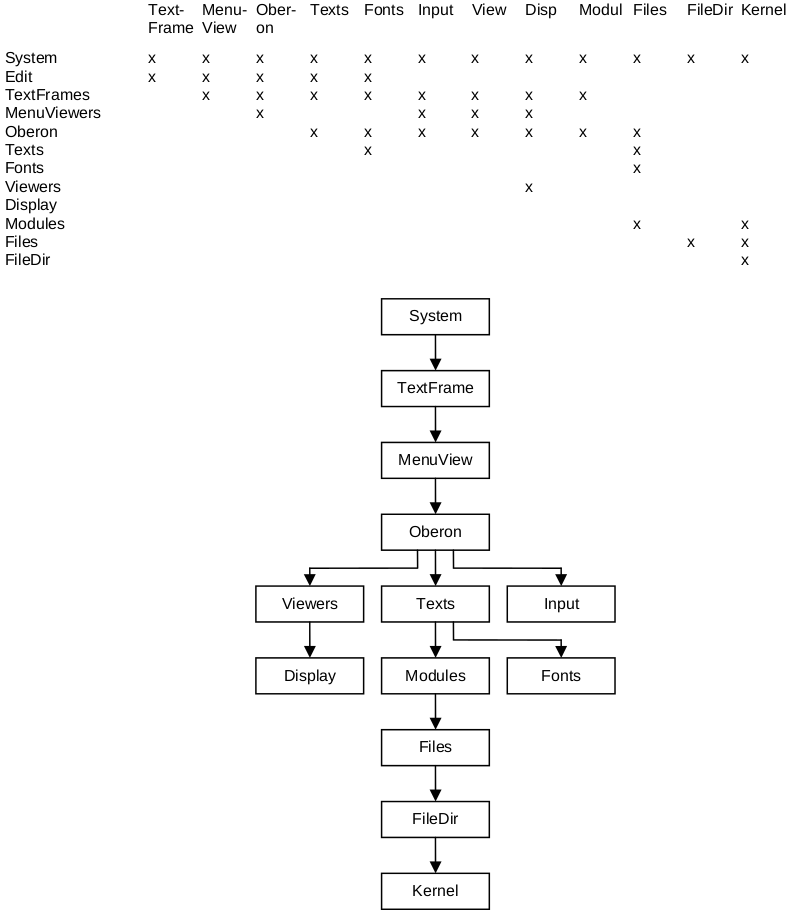
\includegraphics[width=.95\textwidth]{i/2.png}
  \caption{The structure of the Oberon core}
  \label{fig:structure}
\end{figure}

Module names in the plural form typically indicate the definition of an abstract data type
in the module. The type is exported together with the pertinent operations. Examples are
\verb|Files|, \verb|Modules|, \verb|Fonts|, \verb|Texts|, \verb|Viewers|, \verb|MenuViewers|,
and \verb|TextFrames|. Modules whose names are in singular form typically denote a resource
that the module manages, be it a global variable or a device. The variable or the device is
itself hidden (not exported) and becomes accessible through the module's exported procedures.
Examples are all device drivers, \verb|Input| for keyboard and mouse, \verb|Kernel| for
memory and disk, and \verb|Display|. Exceptions are the command modules whose name is mostly
chosen according to the activity they primarily represent, like \verb|System|, and \verb|Edit|.

\verb|Oberon| is, as already mentioned, the heart of the system containing the central loop
to which control returns after each command interpretation, independent of whether it
terminates normally or abnormally. \verb|Oberon| exports several procedures of auxiliary
nature, but primarily also the one allowing the invocation of commands (\verb|Call|) and
access to the command's parameter text through variable \verb|Oberon.Par|. Furthermore, it
contains global, exported variables: the log text. The log text typically serves to issue
prompts and short failure reports of commands. The text is displayed in a log viewer that
is automatically opened when module \verb|System| is initialized. \verb|Oberon| furthermore
contains the 2 markers used globally on the display, the \textbf{mouse cursor} and the
\textbf{star pointer}. It exports procedures to draw and to erase them, and allows the
installation of different patterns for them.

The system shown in Fig \ref{fig:structure} basically contains facilities for generating
and editing texts, and for storing them in the FS. All other functions are performed by
modules that must be added in the usual way by module loading on demand. This includes,
notably, the compiler, network communication, document editors, and all sorts of programs
designed by users. The high priority given in the system's conception to modularity, to
avoid unnecessary frills, and to concentrate on the indispensable in the core, has resulted
in a system of remarkable compactness. Although this property may be regarded as of little
importance in this era of falling costs of large memories, we consider it to be highly
essential. We merely should like to draw the reader's attention to the correlation between
a systems' size and its reliability. Also, we do not consider it as good engineering practice
to consume a resource lavishly just because it happens to be cheap. The following table lists
the core's modules and the major application modules, and it indicates the size of code
(in words) and static variables (in bytes) and, the number of source program lines.
\begin{table}[p]
  \centering
  \begin{tabular}{l r r r}
    module        & code  & data  & lines \\\hline
    Kernel        &  1123 &  8244 &  263  \\
    FileDir       &  1963 &    60 &  352  \\
    Files         &  2360 &   148 &  505  \\
    Modules       &  1214 &   112 &  226  \\
    Input         &   186 &    32 &   79  \\ 
    Fonts         &   628 &    56 &  115  \\
    Display       &  1033 &    84 &  190  \\
    Viewers       &  1324 &   104 &  206  \\
    Texts         &  2906 &   204 &  537  \\
    Oberon        &  1679 &   288 &  410  \\
    MenuViewers   &  1513 &    56 &  208  \\  
    TextFrames    &  5786 &   292 &  874  \\
    System        &  2134 &    72 &  418  \\
    Edit          &  1096 &  1104 &  232  \\\hline
                  & 24945 & 10856 & 4615  \\ [1ex]
    ORS           &  1762 &   992 &  319  \\
    ORB           &  2348 &   408 &  437  \\
    ORG           &  6699 & 34976 & 1125  \\
    ORP           &  5994 &   144 &  974  \\\hline
                  & 16803 & 36520 & 2855  \\ [1ex]
    Graphics      &  3484 &   564 &  685  \\
    GraphicFrames &  2832 &   288 &  498  \\
    Draw          &   690 &    40 &  164  \\
    Rectangles    &   649 &    40 &  118  \\
    Curves        &  1765 &    72 &  241  \\\hline
                  &  9420 &  1004 & 1706  \\
  \end{tabular}
  \caption{Size of Oberon Modules}
  \label{tbl:modsiz}
\end{table}

\section*{References}
\begin{enumerate}
  \item N. Wirth. The programming language Oberon. Software - Practice and Experience 18, 7, (July 1988) 671-690.
  \item M. Reiser and N. Wirth. Programming in Oberon - Steps beyond Pascal and Modula. AddisonWesley, 1992. ISBN 0-201-56543-9
  \item N. Wirth and J. Gutknecht. The Oberon. Software - Practice and Experience, 19, 9 (Sept. 1989), 857-893.
  \item N. Wirth. Ceres-Net: A low-cost computer network. Software - Practice and Experience, 20, 1 (Jan. 1990), 13-24.
  \item M. Reiser. The Oberon - User Guide and Programmer's Manual. Addison-Wesley, 1991. ISBN 0-201-54422-9
\end{enumerate}
